\documentclass[problem]{mcs}

\begin{pcomments}
  \pcomment{CP_missing_card_probability}
  \pcomment{from: S09.cp13m, S07.cp12w}
\end{pcomments}

\pkeywords{
  conditional_probability
  tree_diagram
}

%%%%%%%%%%%%%%%%%%%%%%%%%%%%%%%%%%%%%%%%%%%%%%%%%%%%%%%%%%%%%%%%%%%%%
% Problem starts here
%%%%%%%%%%%%%%%%%%%%%%%%%%%%%%%%%%%%%%%%%%%%%%%%%%%%%%%%%%%%%%%%%%%%%

% F09, S09, S07

\begin{problem}
There are two decks of cards.  One is complete, but the other is
missing the ace of spades.  Suppose you pick one of the two decks with
equal probability and then select a card from that deck uniformly at
random.  What is the probability that you picked the complete deck,
given that you selected the eight of hearts?  Use the four-step method
and a tree diagram.

\begin{solution}
Let $C$ be the event that you pick the complete
deck, and let $H$ be the event that you select the eight of hearts.
In these terms, our aim is to compute:

\begin{equation*}
\prcond{C}{H} = \frac{\pr{C \cap H}}{\pr{H}}
\end{equation*}

A tree diagram is worked out below:

\bigskip
\centerline{\resizebox{!}{3in}{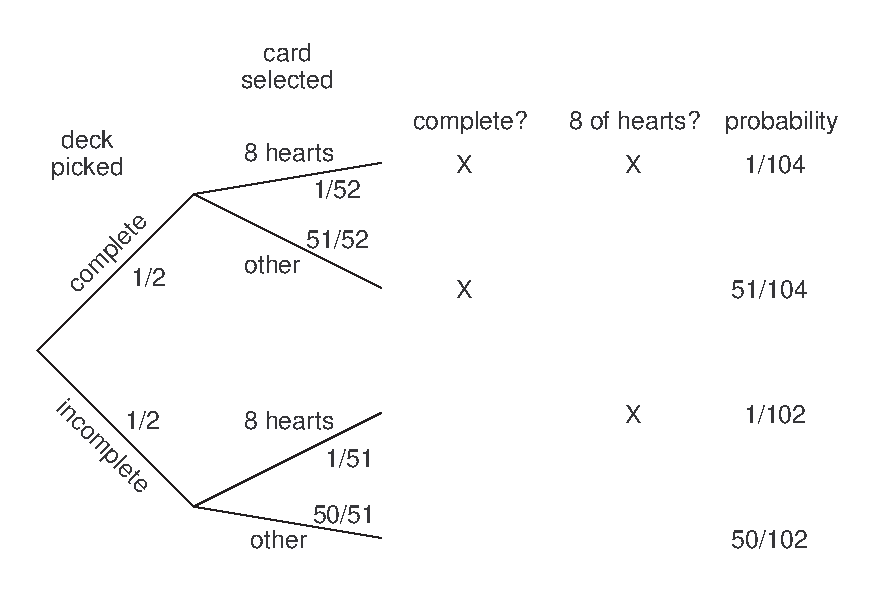
\includegraphics{figures/incomplete-deck}}}
\bigskip

Now we can compute the desired conditional probability as follows:

\begin{align*}
\prcond{C}{H} & = \frac{\pr{C \cap H}}{\pr{H}} \\
              & = \frac{\frac{1}{2} \cdot \frac{1}{52}}
                       {\frac{1}{2} \cdot \frac{1}{52} +
                        \frac{1}{2} \cdot \frac{1}{51}} \\
              & = \frac{51}{103} \\
              & = 0.495146\ldots
\end{align*}

Thus, if you selected the eight of hearts, then the deck you picked is
less likely to be the complete one.  It's worth thinking about how you
might have arrived at this final conclusion without going through the
detailed calculation.

\end{solution}
\end{problem}

%%%%%%%%%%%%%%%%%%%%%%%%%%%%%%%%%%%%%%%%%%%%%%%%%%%%%%%%%%%%%%%%%%%%%
% Problem ends here
%%%%%%%%%%%%%%%%%%%%%%%%%%%%%%%%%%%%%%%%%%%%%%%%%%%%%%%%%%%%%%%%%%%%%

\endinput
